\chapter{Mejora de la precisión en WR} \label{cap:reloj}

El capítulo anterior ha tratado el sistema desde el punto de vista del 
\textit{firmware}, es decir, la parte en lógica reconfigurable y el 
\textit{software} que se ejecuta en el procesador. Para tener una visión 
completa falta analizar el sistema de relojes encargado de la generación de la 
señal fundamental que mantiene la sincronización en cada dispositivo.

El nuevo diseño basado en SoC-FPGA descrito en el capítulo anterior permite 
incluir una configuración del sistema de reloj flexible que se puede adaptar y 
programar de forma sencilla gracias al nuevo soporte del \textit{Processing 
System} para configurar los elementos \textit{hardware} aún cuando la FPGA no 
ha entrado en funcionamiento. Cambiar la configuración del sistema de reloj era 
posible anteriormente pero requería del soporte de elementos externos ya que si 
se cambia algo relacionado con el reloj de referencia usado por la lógica de la 
FPGA, esta deja de funcionar. 

El algoritmo encargado del cálculo del desfase entre relojes en WR consta de un 
bucle de control, tipo Proporcional Integral (PI), implementado 
en sw y HDL que calcula la 
diferencia en frecuencia y fase del oscilador local con respecto al del nodo 
maestro. Este bucle de control calcula una serie de valores de consigna cuyo 
objetivo es corregir la frecuencia de oscilación del reloj local para ajustarse 
al maestro. Esto se realiza en la electrónica externa a la FPGA en un sistema 
formado por un conversor digital/analógico (DAC), un oscilador controlado por 
tensión (VCXO) y un \gls{pll} que se conectan como muestra la Figura 
\ref{fig:wrclk}.

El nuevo sistema de relojes incluido en el WR-ZEN se muestra en la Figura 
\ref{fig:clknewschema}. En él se pueden observar la inclusión de nuevos 
elementos como un PLL extra en el camino de la referencia principal. Esta 
configuración no está pensada para tener dos PLL en cadena (LMK03806 y 
AD9516-4), si no que se aprovecha una característica del primer PLL para 
distribuir la referencia que le entra a otros componentes sin influir de forma 
negativa en su perfil de ruido. Lo que pretende esta configuración es 
flexibilidad el diseño. Mientras que el LMK03806 tiene unas características de 
ruido muy buenas que permiten disminuir el ruido \textit{suelo}, el PLL 
AD9516-4 ofrece una serie de características que son de bastante utilidad como 
desfases programables para sus salidas. De esta manera se cubren distintos 
tipos de aplicaciones (bajo ruido y las que requieren gran flexibilidad) sin 
necesitar una modificación del PCB. Además se ha registrado la salida de PPS lo 
que consigue que dicha señal presente el perfil de ruido del reloj con el que 
se registra, aumentando así en gran manera su estabilidad frente a la versión 
sin registrar de otros dispositivos WR. Por último se incluye otra mejora 
relevante en el área del módulo para la entrada de una frecuencia externa para 
el modo GM, pero se hará referencia a ello en la sección \ref{sec:gm}.

\begin{figure}
	\centering
	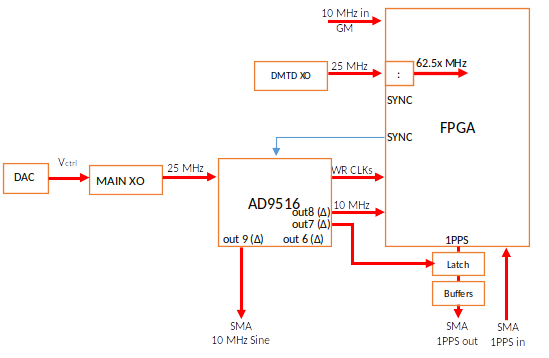
\includegraphics[width=0.7\linewidth]{imagenes/wrclk}
	\caption[Esquema del sistema de reloj en WR]{Esta figura muestra un 
	diagrama de bloques de los componentes principales de la electrónica de 
	relojes para un dispositivo WR.}
	\label{fig:wrclk}
\end{figure}

\section{Caracterización de la nueva plataforma basada en SoC}

El nuevo diseño basado en SoC incluido en el WR-ZEN presenta una serie de 
cambios a nivel de la electrónica de reloj que deben permitir mejorar las 
prestaciones alcanzadas con el resto de dispositivos WR existentes. Dado que 
los cambios en el firmware se encuentran actualmente en desarrollo, y que la 
implementación actual es similar a la presente en el \gls{wrc2p} en el WR-LEN 
la hipótesis de partida es que el rendimiento alcanzado con este nuevo 
dispositivo debe ser almenos equivalente al del WR-LEN. Cumpliendo dicha 
hipótesis se comprueba que la migración a la nueva plataforma no ha supuesto 
ninguna penalización en rendimiento aún cuando la implementación actual no 
aprovecha al máximo todas las ventajas de la nueva plataforma.

Por otro lado se espera que la estabilidad base (es decir sin WR en 
funcionamiento) de la nueva tarjeta sea mayor al resto de equipos actuales como 
el \gls{wrs}, que se usará como modelo de referencia, o el WR-LEN, que también 
será utilizado en las comparativas por incluir la versión de WR basada en el 
\gls{wrc2p}.

Gracias a disponer durante el desarrollo de esta etapa de un medidor de 
\textit{Phase Noise} se ha podido realizar un análisis más exhaustivo que el 
realizado en el capítulo 5. Para caracterizar el nuevo equipo y compararlo con 
los otros dos mencionados anteriormente, se han realizado múltiples medidas de 
ruido de fase para lo cual se ha montado una serie de configuraciones como se 
muestra en la Figura \ref{fig:pnsetup}.




\begin{figure}
	\centering
	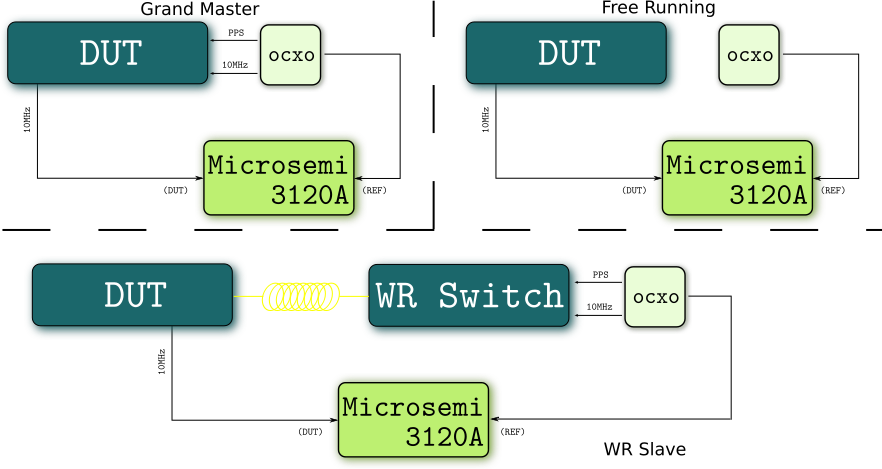
\includegraphics[width=0.7\linewidth]{imagenes/pn_setup}
	\caption[Descripción de la configuración para las pruebas de Phase 
	Noise]{El diagrama muestra las distintas configuraciones utilizadas a la 
	hora de realizar las pruebas para caracterizar el nivel de ruido en los 
	diversos equipos WR. Dependiendo del modo de operación a estudiar se 
	necesita realizar una configuración distinta.}
	\label{fig:pnsetup}
\end{figure}

Para realizar pruebas de ruido de fase se necesita disponer de una referencia 
de reloj lo más estable posible. Esto se debe a que el aparato de medición 
compara dicha señal con la del dispositivo a analizar por lo que cuanto más 
estable sea la señal de referencia, mejores resultados se podrán obtener. En el 
laboratorio se cuenta con un oscilador de tipo OCXO que permite realizar este 
tipo de medidas. En la imagen que acompaña a la Figura \ref{fig:medidapn} se 
puede ver por qué es tan estable este tipo de osciladores: presenta una gran 
capa aislante además de controles que compensan el cambio de temperatura para 
mantener lo más estable posible la frecuencia. A su lado también se puede ver 
un GPSDO que se utiliza en algunas ocasiones como referencia en para este tipo 
de pruebas.

\begin{figure}
	\centering
	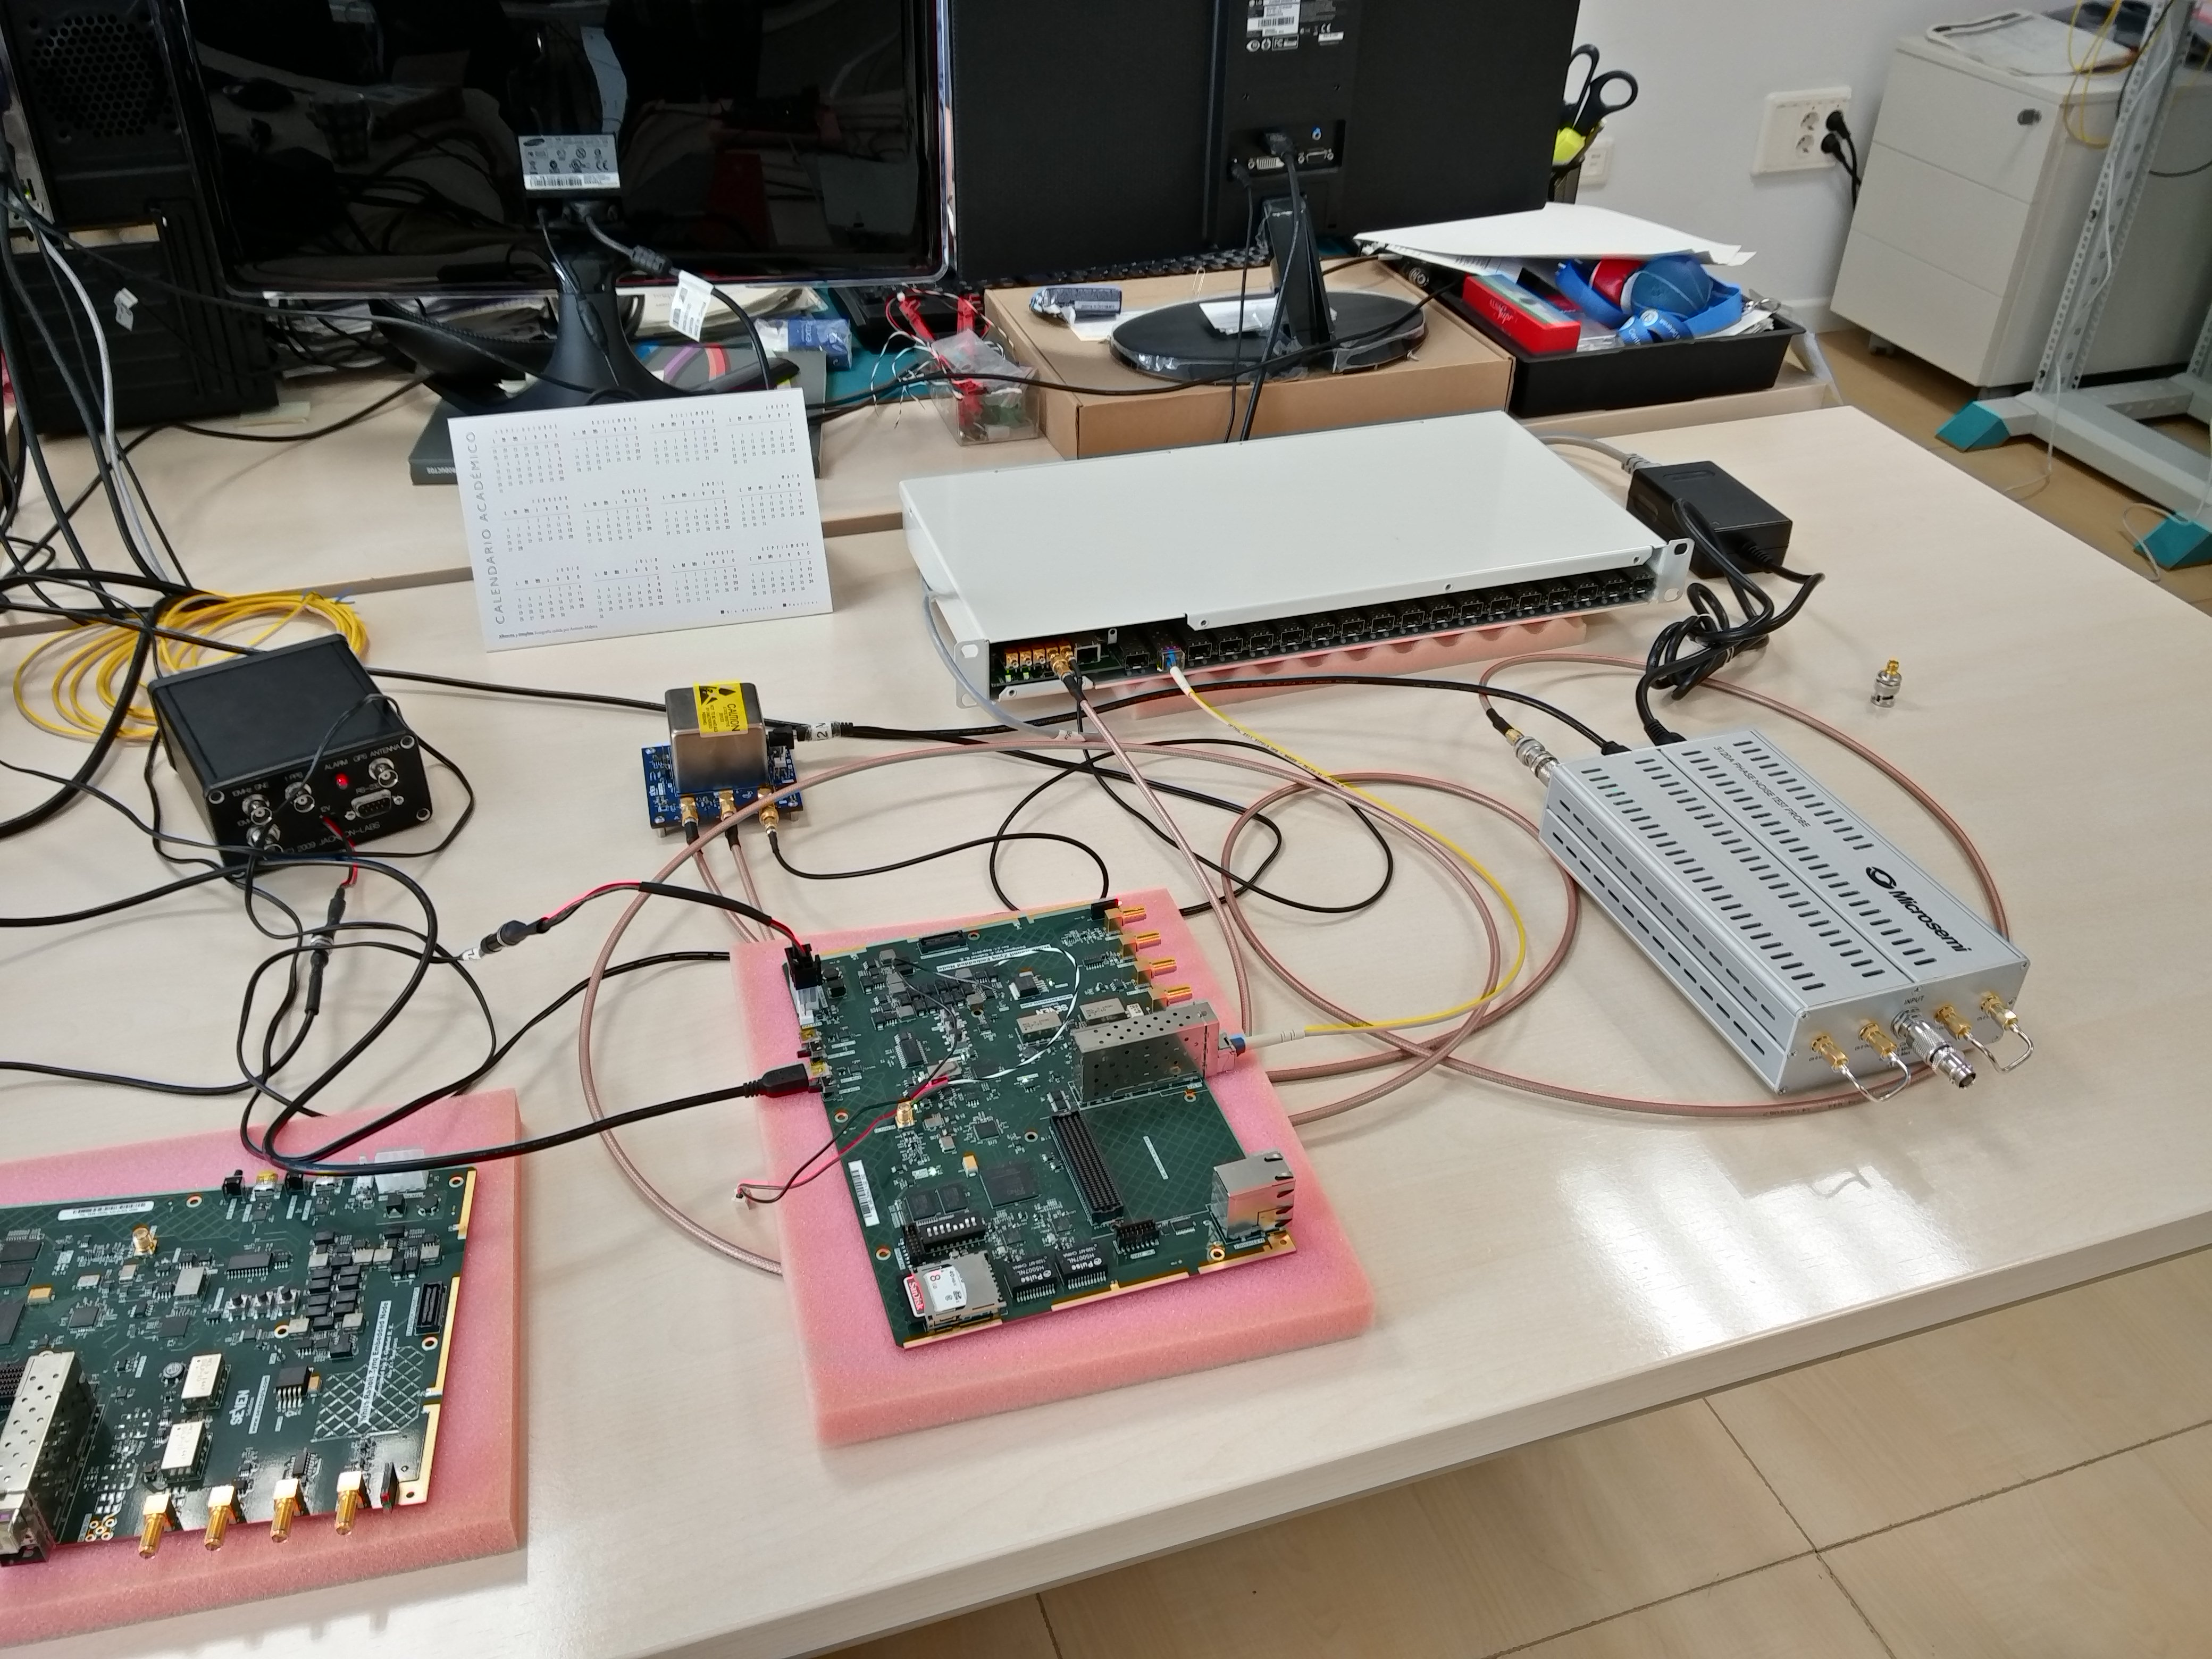
\includegraphics[width=0.7\linewidth]{imagenes/medida_pn}
	\caption[Imagen de la toma de medidas de \textit{Phase Noise}]{La imagen 
	muestra los equipos utilizados para realizar las pruebas de ruido.}
	\label{fig:medidapn}
\end{figure}

Los primeros resultados obtenidos caracterizan el ruido de fase para la 
frecuencia de salida de 10 MHz, generada a partir de la frecuencia de 
referencia disciplinada por WR, para el WR-ZEN. 

\begin{figure}
	\centering
	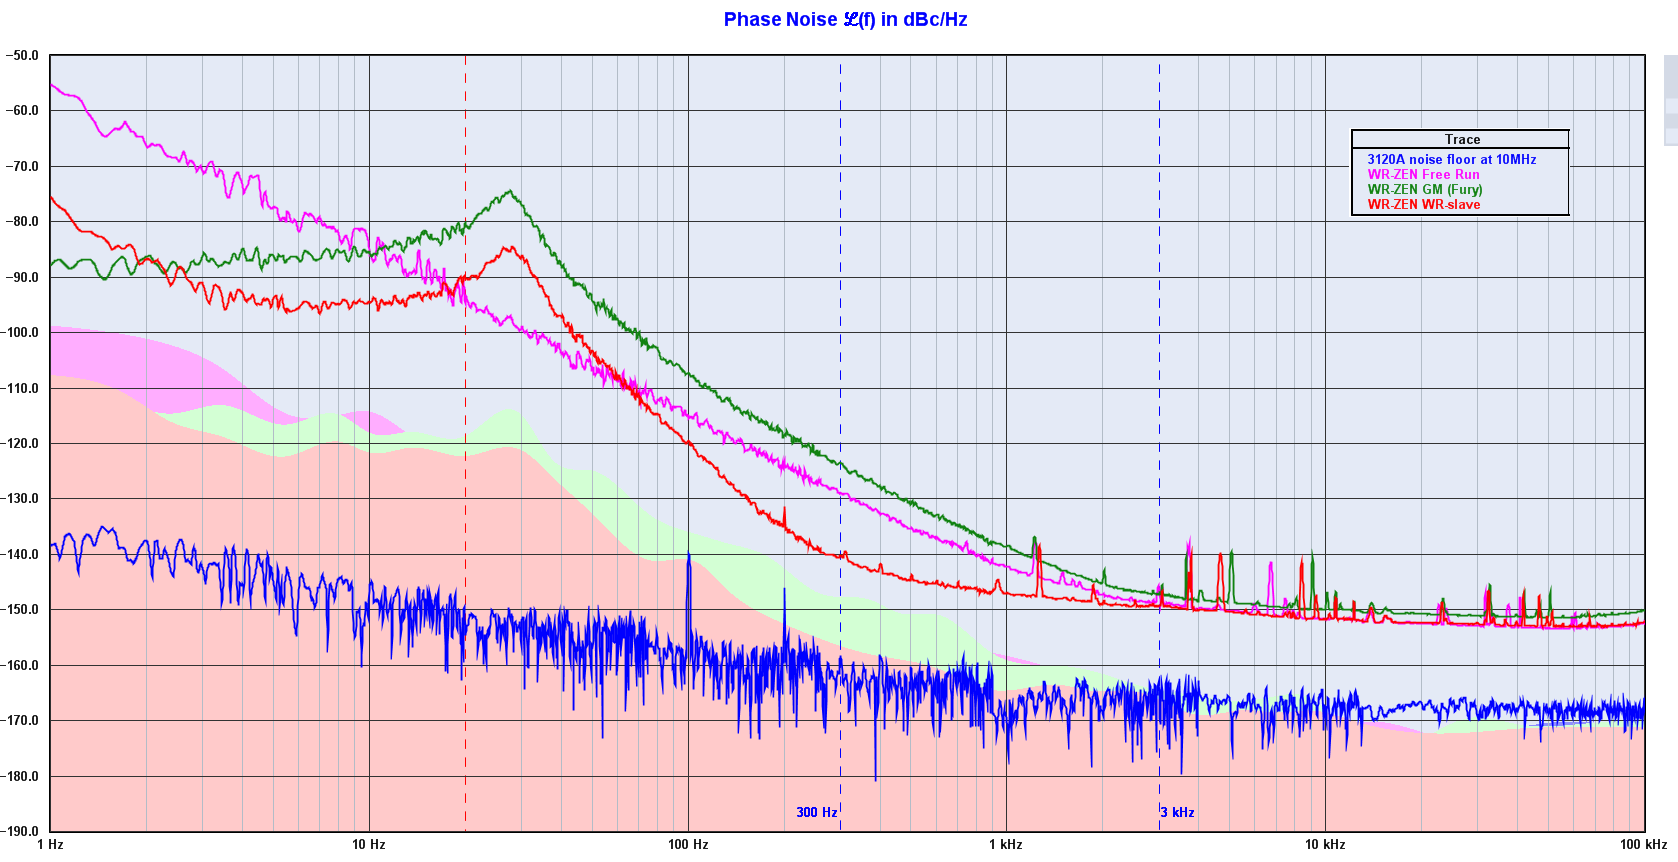
\includegraphics[width=\linewidth]{imagenes/wrzenpn}
	\caption[Gráfico de ruido de fase para el WR-ZEN]{En este gráfico se 
	incluyen los resultados de las medidas de ruido de fase para caracterizar 
	el nivel de ruido presente en el equipo WR-ZEN en los tres modos de 
	operación posibles: maestro \textit{free-running}, maestro GM y nodo 
	esclavo.}
	\label{fig:wrzenpn}
\end{figure}

De forma resumida se comentan los aspectos clave de la información que se puede 
extraer de este tipo de medidas. La línea azul corresponde al ruido base que 
tiene el aparato, es decir, usando el 3120A no se puede medir señales que 
presenten un nivel de ruido inferior al delimitado por la línea azul. Para 
obtenerlo se utiliza el reloj de referencia y mediante el uso de un conector en 
T se divide la señal para usarla como referencia y como señal para el 
dispositivo a medir (\textit{Device Under Test}, DUT). La línea rosa 
corresponde al modo maestro \textit{free running} (la referencia global es su 
propio oscilador local). Las líneas verde y roja corresponden a los modos GM y 
esclavo respectivamente. Se observa el diagrama de Bode típico de un filtro 
paso-bajo. El bucle de control de WR actúa como un filtro que responde ante 
cambios de baja frecuencia sobre la referencia y elimina los producidos en alta 
frecuencia. La frecuencia de corte del filtro se sitúa en torno a los 30 Hz 
como se puede ver en el gráfico. El perfil de ruido final (suelo) que muestra 
el diagrama en \textit{offsets} de alta frecuencia viene limitado por las 
características del PLL utilizado para generar las frecuencias usadas en WR a 
partir del XO de referencia.

\begin{figure}
	\centering
	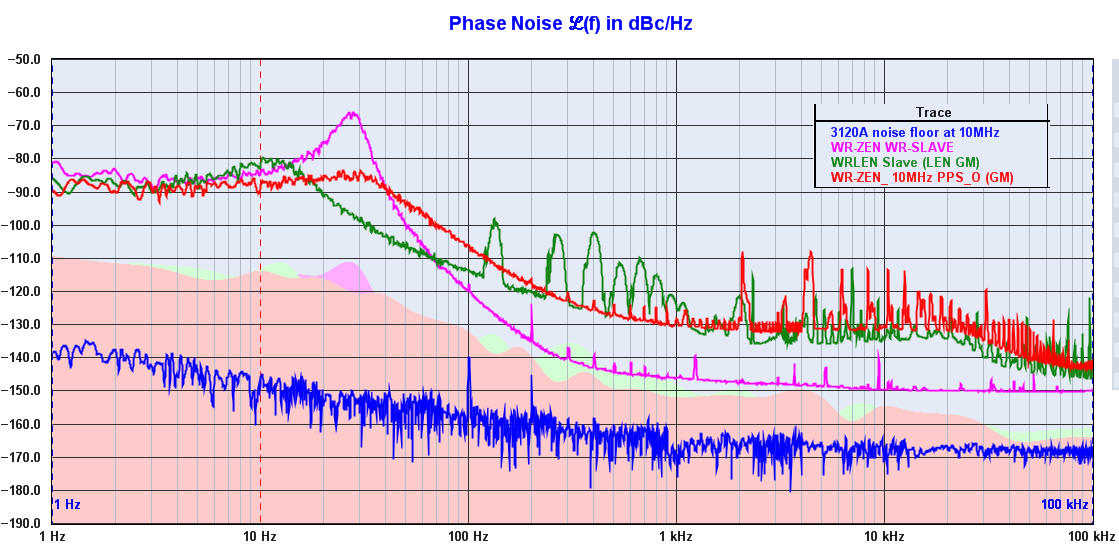
\includegraphics[width=\linewidth]{imagenes/zen_len_comp}
	\caption[Comparativa de \textit{Phase Noise} entre WR-ZEN y WR-LEN]{Este 
		gráfico acompaña una comparativa para los modos esclavo entre el WR-ZEN 
		y 
		el WR-LEN. Además se incluye (línea roja) el resultado de algunas 
		mejoras 
		en el WR-ZEN.}
	\label{fig:zenlencomp}
\end{figure}

\section{Comparativa con otros equipos WR}

Para verificar que la migración a la plataforma Zynq del \gls{wrc2p} y los 
cambios realizados en la electrónica del sistema de reloj no presentan 
problemas se han realizado una serie de medidas de forma similar a las ya 
realizadas para el WR-ZEN (versión de \textit{hw} 2) de manera que se pueda 
comprobar las hipótesis 
planteadas al principio y comprobar que el nuevo desarrollo funciona 
correctamente.

El \gls{wrs} se ha utilizado ya que representa el dispositivo de referencia en 
el mundo \gls{wr}. Las medidas de ruido de fase se han tomado siguiendo la 
misma configuración mostrada en la Figura \ref{fig:pnsetup}. Los resultados se 
acompañan en la Figura \ref{fig:compall}. Para calcular el \textit{jitter} en 
unidades de tiempo se integra el área correspondiente a cada gráfica con 
límites en 1 Hz y 100 kHz, los valores obtenidos se encuentran en la Tabla 
\ref{fig:compall}. 

\begin{figure}
	\centering
	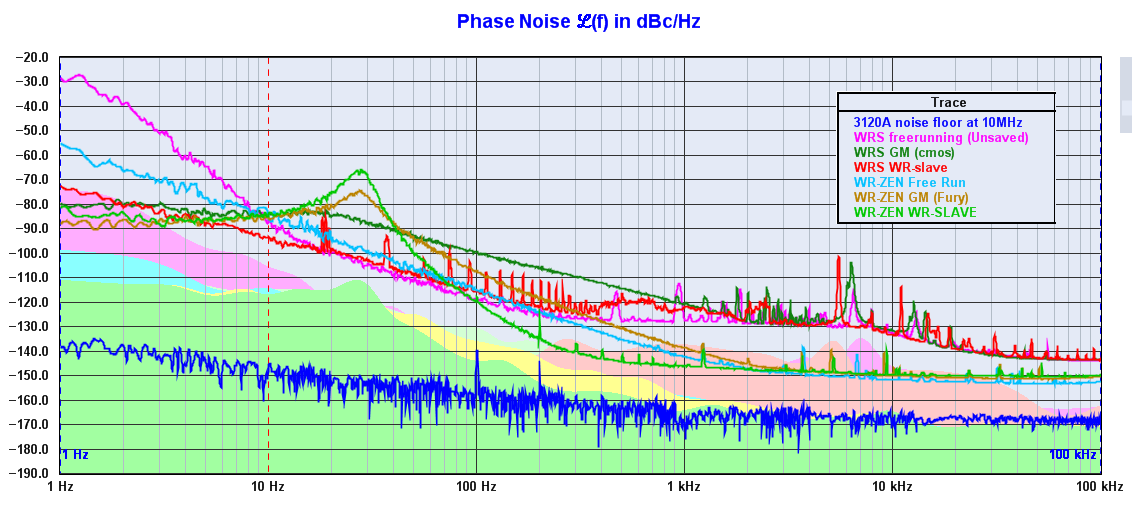
\includegraphics[width=\linewidth]{imagenes/comp_all}
	\caption[Comparativa de \textit{Phase Noise} entre WRS y WR-ZEN]{En este 
	gráfico se muestra la comparativa de ruido de fase entre WRS y WR-ZEN en 
	los tres modos de funcionamiento: maestro \textit{free-running}, maestro GM 
	y esclavo.}
	\label{fig:compall}
\end{figure}

Los resultados muestran que aún queda trabajo por hacer para conseguir el 
objetivo de mejorar las prestaciones para el nodo WR-ZEN. Si se observa los 
perfiles de ruido correspondientes a el modo \textit{free running} se constata 
una gran mejora en la estabilidad gracias a la incorporación de un oscilador 
mucho más estable en el WR-ZEN. Sin embargo, para el resto de gráficas se 
observa una mejor estabilidad en el WRS.

\begin{table}
	% increase table row spacing, adjust to taste
	\renewcommand{\arraystretch}{1.3}
	% if using array.sty, it might be a good idea to tweak the value of
	% \extrarowheight as needed to properly center the text within the cells
	\caption{Valores RMS \textit{jitter} para los resultados de la Figura 
	\ref{fig:compall}.}
	\label{tab:compall}
	\centering
	% Some packages, such as MDW tools, offer better commands for making tables
	% than the plain LaTeX2e tabular which is used here.
	\begin{tabular}{|c||c|}
		\hline
		Dispositivo (modo) & RMS Jitter 1Hz-100kHz (ps) \\
		\hline
		WR-ZEN maestro \textit{free-running} & 25 \\
		\hline
		WRS maestro \textit{free-running} & 620 \\
		\hline
		WR-ZEN maestro GM & 14 \\
		\hline
		WRS maestro GM & 9.4 \\
		\hline
		WR-ZEN esclavo & 30 \\
		\hline
		WRS eclavo & 5.6 \\
		\hline
	\end{tabular}
\end{table}

Para determinar que está limitando mejorar el rendimiento obtenidos por el WRS 
se ha realizado una labor de análisis de los distintos componentes que 
intervienen en el sistema de sincronización. Las conclusiones a las que se ha 
llegado han sido que se necesita optimizar los parámetros del bucle de control 
PI en el WR-ZEN además de adaptar ciertos elementos en la circuitería relativa 
al sistema de reloj. Todo ello viene motivado por los cambios que se han 
realizado en el \textit{hw} con respecto al sistema de referencia utilizado en 
WR.

La Figura \ref{fig:zenlencomp} muestra una pequeña comparativa entre dos nodos 
que incluyen la implementación \gls{wrc2p} en modo esclavo. Según la hipótesis 
de partida, el resultado para ambos debería ser equivalente pues el algoritmo 
de control ha sido migrado sin realizar más cambios que los necesarios para 
ajustarse a la nueva plataforma Zynq. Como en el caso anterior de la 
comparativa con el WRS, el WR-ZEN presenta un rendimiento inferior. Tras la 
labor de análisis se determinó que el \textit{overshoot} visto en torno 20 Hz 
se debía a un cálculo incorrecto en un filtro RC que se encuentra a la salida 
del oscilador principal. Tras modificar el circuito de manera experimental en 
el laboratorio se consiguió reducir dicho fenómeno obteniendo los resultados 
correspondientes a la línea roja de la Figura \ref{fig:zenlencomp}.

\begin{figure}
	\centering
	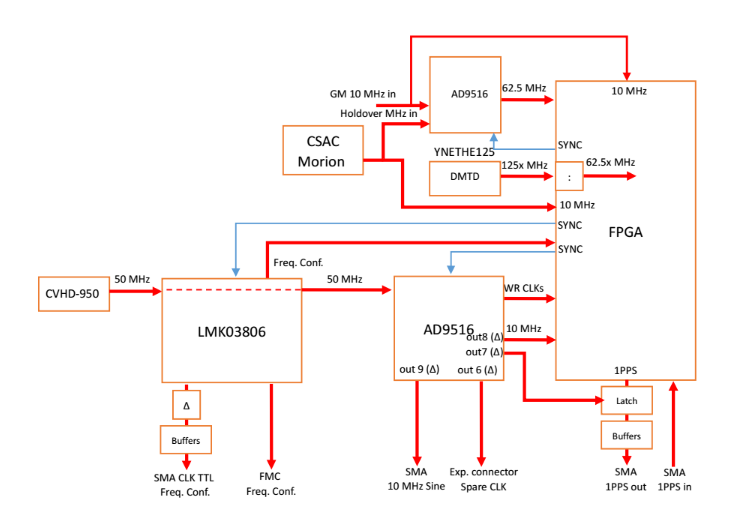
\includegraphics[width=\linewidth]{imagenes/clknewschema}
	\caption[Nuevo esquema de reloj incluido en el WR-ZEN v3.0]{El nuevo 
		esquema de reloj incluido en el WR-ZEN v3.0 incluye las mejoras 
		desarrolladas en el CERN para el modo GM con el PLL externo. Además se 
		pueden apreciar otros cambios con respecto a la electrónica de reloj 
		tradicional.}
	\label{fig:clknewschema}
\end{figure}

Inicialmente había una diferencia en RMS \textit{jitter} entre ambos equipos de 
22.3 ps, y tras el cambio del filtro RC se ha conseguido bajar a 0.8 ps lo que 
equipara prácticamente a ambos dispositivos en rendimiento. Sin embargo, 
gracias a las mejoras realizadas en el \textit{hw} del WR-ZEN el valor de 
\textit{jitter} debería ser menor si se compara con el WR-LEN. En la figura se 
aprecia como el ancho de banda del bucle PI en el caso del WR-ZEN es mayor, 
influyendo en el valor final de RMS \textit{jitter}. La zona fuera del bucle de 
control (alta frecuencia) es mucho más limpia como cabía esperar y no presenta 
el nivel de ruido que si se observa en el caso del WR-LEN.

\section{Línea actual de mejora} \label{sec:gm}


La línea de investigación que se sigue actualmente se centra en mejorar los 
elementos cuyo nivel de ruido limitan la mejora global del sistema. Uno de los 
aspectos clave es el rendimiento alcanzable por el modo \acrlong{gm}. Si 
recordamos en los capítulos iniciales se hace referencia al interés por usar WR 
en centros de metrología (entre otros) para poder distribuir sus costosas y muy 
estables referencias de tiempo a otras instituciones. Sin embargo, actualmente 
el nivel de ruido presente en la electrónica de control utilizada para el modo 
GM presenta una limitación importante en cuanto a rendimiento. Por tanto, no 
sirve de nada tener una referencia muy buena si el sistema utilizado para 
distribuirla la empeora demasiado. 

Este movimiento está liderado por el CERN \cite{mattia2016-2} que ha realizado 
una serie de modificaciones en la electrónica del WRS para incorporar un nuevo 
sistema de PLL que enlaza la frecuencia externa sin necesidad del sistema usado 
hasta ahora en lógica reconfigurable. En resumen, se prescinde de los elementos 
PLL y de generación de señales de reloj internos de la FPGA en favor de 
componentes externos que ofrecen perfiles mucho más bajos de ruido. Este 
movimiento resta flexibilidad y aumenta el coste a cambio de aumentar 
notablemente el rendimiento del sistema.

\begin{figure}[H]
	\centering
	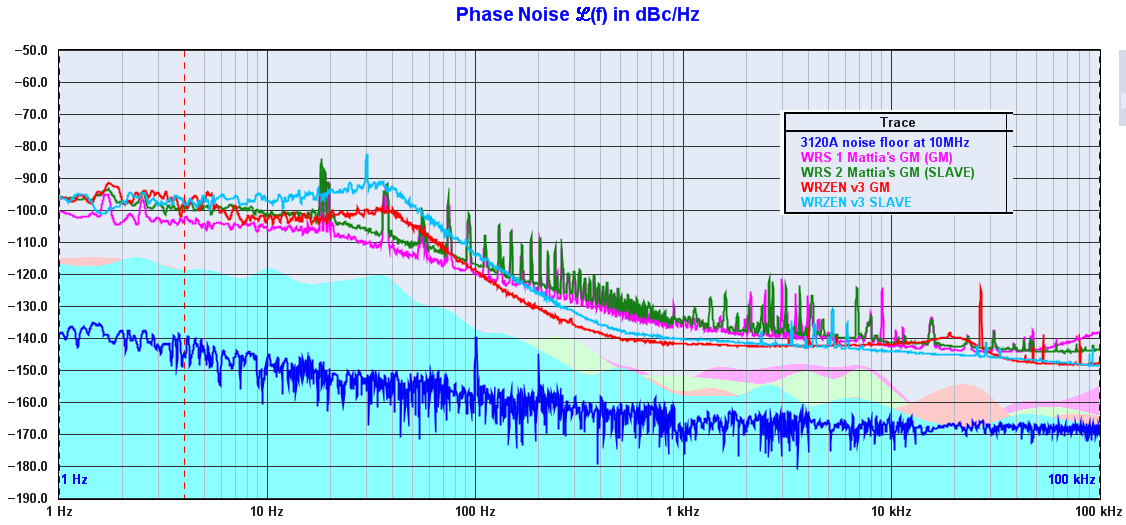
\includegraphics[width=\linewidth]{imagenes/gm_mattia}
	\caption[Resultados de la mejora del modo GM]{Esta gráfica muestra la 
		mejora en el rendimiento obtenido en el WRS y el WR-ZEN gracias a la 
		mejora 
		del modo GM con la incorporación de hw externo a la FPGA para enlazar a 
		la 
		fuente de reloj externa.}
	\label{fig:gmmattia}
\end{figure}

Basándose en el trabajo de Mattia Rizzi en el Cern se han introducido mejoras 
en el diseño del WR-ZEN (de la futura versión de \textit{hw} 3) siguiendo la 
misma línea de incorporar soporte 
\textit{hw} específico para el modo GM. Los resultados se pueden comprobar en 
la Figura \ref{fig:gmmattia} y la Tabla \ref{tab:gmmattia}. Como se puede 
comprobar la mejora ha sido muy relevante, llegando a valores cercanos a 
reducir la barrera del ps. Al igual que en los resultados previos se observa un 
mayor nivel de ruido en el WR-ZEN en comparación con el WRS. Actualmente se 
está realizando una labor de optimización del bucle de control PI en el WR-ZEN 
para conseguir reducir el ancho de banda del bucle y lograr reducir la barrera 
del ps.

\begin{table}
	% increase table row spacing, adjust to taste
	\renewcommand{\arraystretch}{1.3}
	% if using array.sty, it might be a good idea to tweak the value of
	% \extrarowheight as needed to properly center the text within the cells
	\caption{Valores RMS \textit{jitter} para la modificación del modo GM en el 
		WRS y el WR-ZEN.}
	\label{tab:gmmattia}
	\centering
	% Some packages, such as MDW tools, offer better commands for making tables
	% than the plain LaTeX2e tabular which is used here.
	\begin{tabular}{|c||c|}
		\hline
		Dispositivo (modo) & RMS Jitter 1Hz-100kHz (ps) \\
		\hline
		WR-ZEN GM mejorado & 1.7 \\
		\hline
		WRS GM mejorado  & 1.5 \\
		\hline
		WR-ZEN esclavo mejorado & 3.4 \\
		\hline
		WRS esclavo mejorado & 2.0 \\
		\hline
	\end{tabular}
\end{table}

\section{Conclusiones}

Toda la circuitería encargada del sistema de generación y recuperación de la 
referencia de reloj utilizada en WR es un sistema clave si se pretende lograr 
una mejora en el rendimiento alcanzado por este protocolo. Los cambios vistos 
en anteriores capítulos pueden mejorar la flexibilidad del diseño gracias al 
uso de nuevas plataformas basadas en SoC y también pueden lograr cierto nivel 
de mejora en las prestaciones aunque en este apartado la mayor parte del ruido 
del sistema se debe a la circuitería utilizada para el sistema de relojes.

Por ello no basta con realizar cambios en el \textit{firmware} si no que es 
necesario emprender una labor de caracterización y análisis de los componentes 
que intervienen en dicha circuitería. Dada mi formación como informático mi 
contribución a este aspecto se ve más limitada por mi conocimiento de 
electrónica. Sin embargo puedo aportar mi granito de arena colaborando en 
realizar análisis que permitan detectar posibles mejoras que luego serán 
realizadas por los diseñadores de circuitos electrónicos. También es clave la 
caracterización de los equipos ya que permite determinar el rendimiento real 
del sistema comprobando si se han cumplido las hipótesis de diseño iniciales.

Con el diseño del WR-ZEN se buscaba mejorar el rendimiento global para la 
arquitectura de nodo basada en el \textit{wrc2p}, motivo de ello es la 
incorporación de nuevos componentes que sobre el papel ofrecen mejores 
características que los utilizados en los diseños de referencia de WR. Además 
la nueva arquitectura basada en SoC ha permitido realizar un diseño flexible 
que es capaz de adaptar múltiples configuraciones del sistema de reloj para 
conseguir un menor ruido, \textit{offsets} programables, etc. Esta nueva 
configuración es de gran ayuda durante la labor de investigación pues permite 
probar múltiples configuraciones distintas sin necesitar cambios a nivel de 
rediseño de la PCB. 

Sin 
embargo, los resultados obtenidos, aunque son buenos, evidencian el hecho de 
que todavía queda trabajo por hacer. Se ha comprobado que la nueva circuitería 
de reloj ofrece un perfil de ruido más bajo y limpio que en modelos anteriores, 
pero el rendimiento obtenido está todavía por debajo de las expectativas.

Actualmente estoy trabajando en seguir mejorando el rendimiento en el WR-ZEN 
enfocándome en el bucle de control PI para jugar con el ancho de banda del 
mismo para intentar reducir el ruido observado en los resultados anteriores.

\section{Aplicaciones}

Los nodos WR eran típicamente dispositivos muy simples que estaban pensados 
para su uso como parte de un sistema mayor. Ejemplo de ello es la tarjeta SPEC, 
pensada para ser conectada a un puerto PCIe de un PC. Aunque existen nodos como 
el WR-LEN que pueden actuar perfectamente de forma autónoma, a la hora de 
integrar el nodo WR dentro de una aplicación mayor surgen varias deficiencias 
que se han tratado de solventar con la inclusión de la arquitectura basada en 
SoC-FPGA. Sobre todo cabe destacar el alto coste de desarrollo que tiene añadir 
cualquier funcionalidad a la arquitectura de nodo inicial y la falta de 
recursos para hacerlo. Gracias al nuevo diseño muchas más aplicaciones pueden 
adaptar a sus necesidades el diseño actual ya que incluir nuevos protocolos o 
aplicaciones de usuario es relativamente sencillo gracias al soporte de drivers 
y de la capa de abstracción hardware que permiten abstraer a los 
desarrolladores de la implementación de más bajo nivel del sistema.
Así mismo las mejoras realizadas en el ámbito de las prestaciones posibilitan 
la utilización de la tecnología WR en aplicaciones con altos requisitos de 
sincronización, como nuevas instalaciones científicas (SKA por ejemplo) o la 
distribución de frecuencia con limitación al ruido del sistema. La reducción 
del \textit{jitter} del sistema es algo que se está demandando desde el sector 
metrólogico. Estas instituciones necesitan propagar su referencia de tiempo con 
la mínima degradación posible, así que cualquier mejora en este sentido será 
recibida con los brazos abiertos por dicho sector. Por otra parte otro campo 
que se verá beneficiado es el distribución de tiempo con enlaces de muy larga 
distancia, donde también es clave mantener un perfil de ruido bajo para 
compensar el deterioro provocado por la longitud del enlace.

Parte de los resultados obtenidos en este trabajo también se enfocan en la 
escalabilidad y los limites de la tecnología con el foco en aplicaciones menos 
exigentes. Los experimentos han permitido determinar el número máximo de nodos 
que actualmente soporta la implementación basada en \gls{wrc2p} en el WR-LEN, 
cuyos resultados son extrapolables a otros equipos WR gracias al mantenimiento 
de la electrónica de referencia en el dispositivo utilizado para dichas 
pruebas, y además los valores de exactitud en la sincronización en cadenas 
largas de dispositivos. Estos datos son de gran importancia a la hora de elegir 
esta tecnología en aplicaciones con redes con muchos nodos conectados en 
cadena, telecomunicaciones o grandes factorías son ejemplos. 

